\chapter{Project Design}
\vspace{-1cm}
\par This section describes how Project Design serves as the foundational blueprint for developing a software solution. It outlines the overall structure, essential features, and technical specifications, guiding the entire development process. The Features and Functionality part details the specific capabilities and user-facing components of the project, explaining what the system will do and how users will interact with it. This comprehensive breakdown of core modules ensures the final product is a centralized and efficient platform that aligns with the project’s goals and user needs. 

\section{Features and Functionality}
\begin{itemize}
\item \textbf{Automatic Data Analysis \& Preprocessing:}

The platform automatically analyzes the structure of uploaded datasets and performs necessary preprocessing steps to prepare the data for training. This includes handling missing values, formatting features, and ensuring the dataset is clean and suitable for machine learning workflows. By automating this process, it reduces manual effort and allows users to focus more on model building rather than data preparation.\\

\item \textbf{Multi-Model Training:}

The system supports training multiple machine learning models simultaneously based on the given dataset. This enables users to explore different algorithms without manually configuring each one, ensuring a comprehensive approach to model development and improving the chances of achieving optimal performance.\\

\item \textbf{Best Model Selection:}

After training multiple models, the platform automatically evaluates their performance and selects the most accurate one. This eliminates the need for manual comparison and ensures that the best-performing model is chosen for further use.\\

\item \textbf{Model Export (.pkl):}

Once the best model is selected, the system generates a reusable \texttt{.pkl} file. This file can be easily integrated into applications or deployed in real-world systems, making the transition from development to production seamless.\\

\item \textbf{Prediction Interface:}

The platform provides a simple and user-friendly interface where users can input data and receive predictions from the trained model. This makes machine learning accessible even to users with minimal technical expertise.\\

\item \textbf{Dataset Upload \& Processing:}

Users can upload their datasets directly to the platform, where the system processes and prepares the data for model training. This feature ensures a smooth and efficient workflow from data ingestion to model development.\\

\item \textbf{Automatic Model Training:}

Based on the type and structure of the dataset, the platform automatically initiates training using suitable machine learning models. This reduces the need for manual configuration and speeds up the development process.\\

\item \textbf{Model Evaluation \& Selection:}

The system evaluates all trained models using relevant performance metrics and compares their results. It then selects the best-performing model, ensuring accuracy and reliability in predictions.\\

\item \textbf{Model Deployment (.pkl):}

The selected model is converted into a deployable \texttt{.pkl} file, allowing users to integrate it into real-world applications, APIs, or systems with ease.\\

\item \textbf{Prediction System:}

The platform enables users to input new data and obtain predictions through an intuitive interface. This feature ensures that the trained model can be effectively used for practical decision-making and real-time applications.\\


\end{itemize}

\vspace{10 cm} 

\section{System Architecture}
\begin{figure}[H]
    \centering
    % Image ko -90 degree rotate kiya gaya hai
    % NOTE: width aur height ki values ko aapas mein badal diya gaya hai
    \fbox{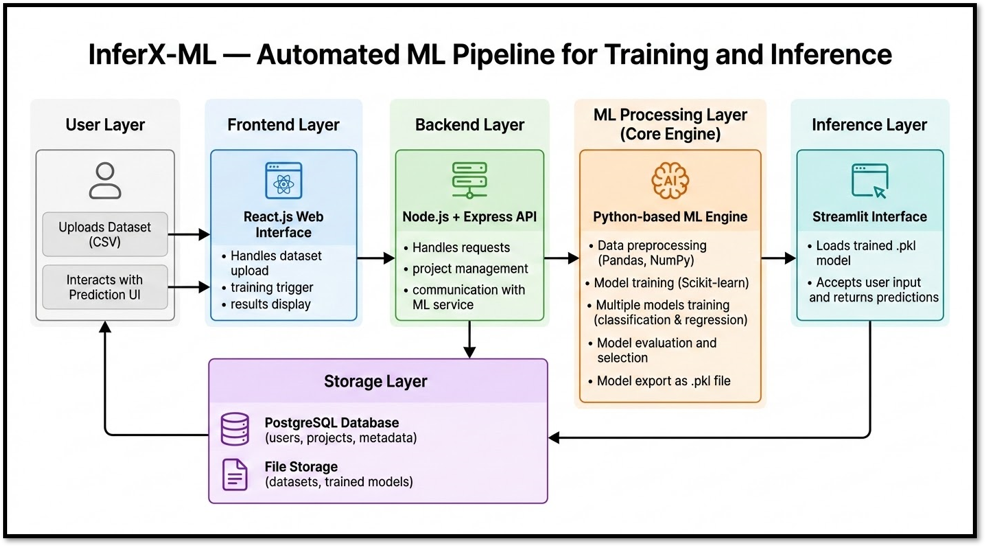
\includegraphics[width=16cm, height=10cm]{images/Designer.png}}
    \caption{System Architecture of InferX-ML}
    \label{fig:image1}
    \vspace{0.2cm}
    \parbox{\textwidth}{\small The diagram illustrates the architecture of InferX-ML, an automated machine learning pipeline that streamlines training and inference. It shows the flow from user interaction through frontend and backend layers to a Python-based ML engine, which handles data preprocessing, model training, and selection. The system stores data and models efficiently and provides predictions through an inference layer using a simple user interface.}
\end{figure}

\vspace{10 cm}

\section{DFD (Data Flow Diagrams)}
\begin{figure}[H]
    \centering
    \fbox{\includegraphics[width=17cm, height=3.5cm]{images/dfd-0.png}}
    \caption{Data flow Diagram of InferX-ML (Level 0)}
    \label{fig:image2}
 \vspace{0.2cm} % Adds a small space after the caption
    \parbox{\textwidth}{\small This Data Flow Diagram (DFD) at Level 0 represents the overall system context for the InferX-ML platform, where the User interacts with the central system to upload data, train models, and generate predictions, while the platform processes requests through its backend, ML engine, and storage, and integrates with external AI services like the Gemini API to deliver insights.}
\end{figure}

\begin{figure}[H]
    \centering
    \fbox{\includegraphics[width=17cm, height=7cm]{images/dfd-2.png}}
    \caption{Data flow Diagram of InferX-ML  (Level 1)}
    \label{fig:image2}
\vspace{0.2cm} % Adds a small space after the caption
    \parbox{\textwidth}{\small This Data Flow Diagram (DFD) at Level 1 represents the detailed workflow of the InferX-ML platform, where the User interacts with modules like authentication, dataset management, training orchestration, and the ML engine to build and deploy models, while data and models are stored in PostgreSQL and MinIO, and the AI Insight Layer integrates with the Gemini API to generate explainable, human-readable insights.}
\end{figure}

\begin{figure}[H]
    \centering
    \fbox{\includegraphics[width=17cm, height=5.5cm]{images/dfd-1.png}}
    \caption{Data flow Diagram of InferX-ML (Level 2)}
    \label{fig:image2}
\vspace{0.2cm} % Adds a small space after the caption
    \parbox{\textwidth}{\small This Data Flow Diagram (DFD) at Level 2 represents the modular architecture of the InferX-ML platform, where the User interacts with distinct microservices such as Auth, Dataset Management, Training, ML Engine, and Prediction services, each connected to dedicated storage systems (PostgreSQL and MinIO), while the AI Insight Layer integrates with the Gemini API to generate intelligent insights.
}
\end{figure}

\section{Use Case Diagram}
\begin{figure}[H]
    \centering
    \fbox{\includegraphics[width=15cm, height=20cm]{images/new.png}}
    \caption{Use Case Diagram of InferX-ML}
    \label{fig:img5}
\vspace{0.2cm} % Adds a small space after the caption
    \parbox{\textwidth}{\small A use-case diagram of an AI Model Training Platform showing subsystems like authentication, dataset management, training, model management, and prediction.
It illustrates how a user interacts with these components and integrates external AI services (Gemini API) for analysis and insights.}
\end{figure}

